%!TEX root = thesis.tex
\section{Data Steam Processing System Technology Overview}
\label{sec:overview}

This chapter describes the choices for data stream processing systems (DSPS) in which the pipeline for the Monash University
Institute of Railway Technology will be built, along with the methods which will be used for evaluating the different
technologies used. As identified in the the previous chapter, a number of relatively new DSPS technologies exist and have been in use
in different projects at different companies. Here we will look at more of an overview of the possibilities they offer
in terms of programming interfaces. Furthermore, we will outline the testing parameters that will be used in a later
chapter to evaluate the usage of each technology, highlighting both quantitative performance-based metrics as well as
qualitative metrics looking at the ease of programmability from the point-of-view of the DSPS programmer.

This chapter will first start with a look at the choices in DSPS technology which will be used further in the project,
in~\sectref{sub:dsps_technology_choices}, before going into the evaluation methods and approach in~\sectref{sub:evaluation_method_approach}.
Finally, we will look at an overview of the testing data in~\sectref{sub:overview_of_the_data}, before concluding in~\sectref{sub:conclusion}.


\subsection{Data Steam Processing System Technology Choices} % (fold)
\label{sub:dsps_technology_choices}

The DSPS technologies that have been chosen to be focused on in this sub-project include the following:

\begin{itemize}
  \item Samza
  \item Storm
  \item Spark Streaming
\end{itemize}

Literature concerning these DSPS technologies have been covered in~\sectref{sub:realtime_data_processing}, however
we will look into more depth into the systems regarding their usage from the programmer's point-of-view. Note that
in the previous chapter, a further DSPS technology, S4, was covered, however due to its notes decline in usage and
development in the chapter, it has been decided to omit the use of the technology from this project.


\subsubsection{Samza Programming} % (fold)
\label{ssub:samza_programming}

\textit{Note that the majority of the content in this section is sourced from the official Samza 0.9 documentation.}~\cite{Samza6:online}

Samza defines itself as a realtime data processing system which allows the processing of streams made up of immutable
messages of similar type or category. Streams in Samza exist independently of other concepts, allowing themselves to be
\textit{consumed} from or \textit{produced} to by various supported systems. The concepts of consuming and producing refer
to the actions of getting data from a stream and placing data onto a stream, respectively. Samza defines the systems that can be used
for consuming and producing to streams to be any piece of software that implements the stream abstraction. For example,
Kafka, a popular distributed messaging queueing system, is often used to consume and produce to Samza streams. Systems such as these can be
``plugged'' into a Samza project to work with the same streams which native Samza applications are written to work with.

For a Samza programmer, the most important concepts of the overall Samza project to understand are the concepts of the
\textbf{system} and \textbf{task}. In a Samza project, a system exists to produce a particular stream which then can
be processed by a task which consumes it. A task will always then produce output to another stream. Systems and tasks
can then be arranged in a pipeline-like structure allowing a specified type of processing on the messages which travel
on those streams. Hence, it is easy to think of a system as the source of data for an overall Samza project. A very
simple example of such a Samza project is shown in~\figref{fig:samza_overview}.

\begin{figure}[h]
  \centering
  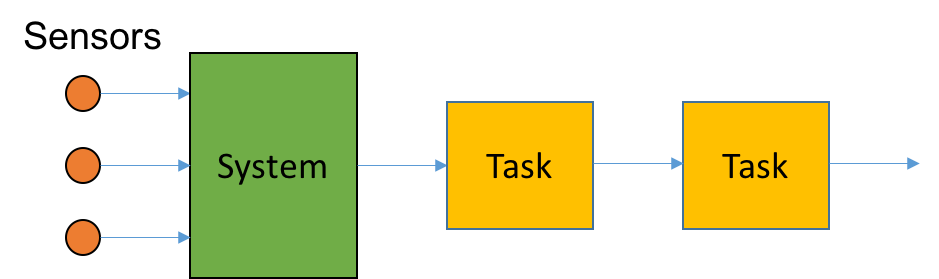
\includegraphics[width=0.8\textwidth]{includes/figures/fig_samza_overview}
  \caption{A simple Samza pipeline showing the roles of the system, task, and stream concepts. Streams are represented
  as arrows.}
  \label{fig:samza_overview}
\end{figure}

When programming a Samza project, interfaces exist for both the system and task concepts through the \texttt{org.apache.samza.system.SystemConsumer}
and \texttt{org.apache.samza.task.StreamTask} Java interfaces. Existing systems exist in the Samza project, and may be
used to produce streams which can then be processed by an implemented \texttt{StreamTask}.

The \texttt{StreamTask} interface is arguably the main interface in which the most important processing will be done in
a Samza project. It requires implementing a single method, \texttt{process}, which passes in an immutable message from the stream
on which the task is configured to consume. These messages are then processed as specified by the programmer before the
result of the processing is wrapped in a message envelope and produced to a stream specified by the programmer.

The streams on which \texttt{StreamTask} implementations consume are specified in a task specific configuration file,
independent to that of the implementation source code. These configuration files offer a range of parameters for the
execution of tasks, each of which are documented\footnote{https://samza.apache.org/learn/documentation/0.9/jobs/configuration-table.html},
however can result in quite verbose and hard to understand configurations files. For each task configuration, a system
needs to be defined that produces to the stream that the task consumes from. These can either be a self-implemented
system, or an existing pluggable system, such as Kafka.

For self-implementation of systems, then \texttt{SystemConsumer} interface requires much more understanding and effort to
implement than that of the \texttt{StreamTask} interface. Methods, such as \texttt{start}, \texttt{stop}, \texttt{register},
and \texttt{poll} need to be implemented, allowing for the producing of messages onto a particular stream. The \texttt{start}
and \texttt{stop} methods simply connect and disconnect the system to the underlying system, while the \texttt{poll}
method takes care of producing any messages from the system. The \texttt{register} method is much more complicated in the
way that it requires registering the implemented system with lower-level components of Samza to integrate the system into
Samza.

Note that, due to Samza's relative infancy to other DSPS technologies, many of these interfaces either completely lack
or offer insufficient documentation. Furthermore, for the same reason, example Samza projects are hard to find. This is
a key factor that will be touched upon in later chapters on evaluating the DSPS technologies.

Samza projects are generally compiled and distributed as JAR files, which may or may not contain project dependencies,
which then can be run directly on installed Samza distributions. Assembly of these JAR files are conventionally performed
through use of Java build automation tools, such as Maven or Gradle.

% subsubsection samza_programming (end)


\subsection{Storm Programming} % (fold)
\label{sub:storm_programming}

% subsection storm_programming (end)


\subsection{Spark Streaming Programming} % (fold)
\label{sub:spark_streaming_programming}

% subsection spark_streaming_programming (end)

% subsection dsps_technology_choices (end)



\subsection{Evaluation Method \& Approach} % (fold)
\label{sub:evaluation_method_approach}

Evaluation will be performed using both qualitative and quantitative methods. The quantitative evaluation methods used will focus
on the benchmarking of various features that are common to each of the technologies, and the comparison of the features that
each technology supports. The qualitative evaluation methods will focus on looking at the differences in ease-of-use,
support for different programming languages and features, and complexity of code written to implement the pipeline.

With looking at the decision of giving a clear recommendation for a particular technology out of the ones we have chosen,
we think it is import to look at both qualitative and quantitative aspects for comparison. These systems are significantly
non-trivial and vastly different in design and usage, however, as they still afford the same possible functionality,
it is very possible to give a properly constructed evaluation of them.


\subsubsection{Quantitative methods} % (fold)
\label{ssub:quantitative_methods}



% subsubsection quantitative_methods (end)


\subsubsection{Qualitative methods} % (fold)
\label{ssub:qualitative_methods}

The qualitative methods used to evaluate the DSPS systems for the pipeline will include the following:

\begin{itemize}
  \item
\end{itemize}

% subsubsection qualitative_methods (end)

% subsection evaluation_method_approach (end)



\subsection{Overview of the data} % (fold)
\label{sub:overview_of_the_data}

As this sub-project focuses on the realtime processing of streaming data, data streams will have to be simulated from
datasets acquired from the Monash IRT team. An initial dataset has been given that includes the following layout of data:

%TODO: table from my other paper

The sample data acquired from the IRT team includes 99\,999 rows of data recorded from each of the mentioned sensors,
organised in a CSV file with headers. This is a general example of how data is currently received and handled by the IRT
team, however in the case of realtime data processing, data would be received in quite a different manner. Rather than
being received in large batches of readings, such as the sample dataset acquired, streams of data may be created from
each particular sensor, delivering data values to the DSPS systems a single value at a time along those streams. Data
is streamed in an asynchronous fashion, and can be simply thought of as DSPS system listens on an incoming stream, and
acts upon any data value whenever they may be received.

Hence, to simulate streaming data from the data samples we have acquired, the DSPS pipeline is constructed to listen on
a particular socket connection for any incoming data. Once a data value is encountered on the connection, it is fed into
the pipeline and processed accordingly while the pipeline continues to listen on the socket for further incoming data.
As the pipeline is constructed in such a way, we can simulate the data being sent out from sensors using a program such
as \texttt{netcat}~\footnote{http://nc110.sourceforge.net/}, where we can pipe data from a file to a particular
socket over a connection.

% subsection overview_of_the_data (end)

\subsection{conclusion} % (fold)
\label{sub:conclusion}

% subsection conclusion (end)
